\documentclass[11pt,a4paper]{article}

\usepackage{classeRapport}
\usepackage{graphicx}
\usepackage{caption} 

\begin{document}

\PageDeGarde	
{snake.jpg} % image sur la page de garde
{Rapport de projet SNAKE I4.2} % titre principal
{Domptez le serpent qui est en vous.} % sous-titre
{Alexandre \textsc{ODIN}\\
Tom \textsc{SIMON}\\
Timothé \textsc{VERSTRAETE}\\
Yassine \textsc{BEN ABDERRAHMANE }\\
Titouan \textsc{VITRAI}\\
Alexandre \textsc{DOUBLET}\vspace{5cm}}
{I4.2 – STPI2 – 2020} % bas de page


\Page{INSALogo} % logo de bas de page (en bas a droite)

\tableofcontents

\clearpage % Pour faire un saut de page propre
\section*{Introduction} % L'astérisque est pour que la section ne soit pas numérotée
\addcontentsline{tod}{section}{Introduction} % Cette commande ajoute la section à la table des matières malgré le fait qu'elle ne soit pas numérotée

   
   
   Dans le cadre du cour de I4.2, nous nous sommes lancé dans la réalisation du jeu SNAKE.  L'objectif de ce projet est d'exploiter l'ensemble de nos compétences acquises au cours de nos formations à l'INSA ainsi qu'utiliser de nouveaux outils introduits en I4.2 tel que git ou le langage \LaTeX{}  pour la rédaction de notre rapport. Face à un tel projet, il était nécessaire dé gérer efficacement nos données. Git est un logiciel de gestion de versions décentralisé. Grace à lui, nous disposions d’un dossier distant, sur lequel nous pouvons travailler à plusieurs.\\
   
   À travers la réalisation du jeu Snake, l'enjeu n'était pas seulement de créer un programme fonctionnel, il fallait professionaliser nos méthodes de travail. Ainsi, nous avons respecté les 4 phases propres à la création d'un programme informatique afin de faire évoluer notre projet méthodiquement.
   
   \begin{enumerate}
    \item La conception globale (les différents types utilisés + analyse decendante)
    \item La conception préliminaire
    \item La conception détaillée
    \item Implementation
    \end{enumerate}
   
  Nous formons un groupe de six personnes. Cela implique une bonne organisation, une répartition du travail efficace, ainsi qu'une bonne coordination des actions, notamment lors de l'utilisation de git. 

\clearpage % Pour faire un saut de page propre

\section{Analyse du projet}
    
    \subsection{Cahier des charges}
        \subsubsection{Description du projet}
        
            Le snake est un jeu qui est devenu un classique à partir du moment où Nokia l'a intégré dans ses produits en 1998. Le principe du jeu est relativement simple. Le joueur contrôle un serpent en lui indiquant 4 directions possibles (en haut,en bas ,à droite, à gauche). Le serpent doit survivre en évitant que sa tête ne touche les murs ou son propre corps. En même temps, il doit manger le maximum de nourriture afin de grandir et d'obtenir le meilleur score possible. Il existe de nombreuses versions de ce jeu mais celle que nous vous proposons est de loin la meilleure.
            
        \subsubsection{Liste des fonctionnalités}\label{sssect:fonctionnalites}
        
            Le rendu final de notre projet comporte les fonctionnalités suivantes:\\
            
            \begin{itemize}
                \item Jeu snake classique avec murs 
                \item Menu principal et sous-menus 
                \item Affichage console + Coloration de l'affichage
                \item Génération spécifique pour chaque objet
                \item Choix de la taille du plateau et choix de la difficulté (Vitesse du serpent)
                \item Mise en place de score
                \item Sauvegarde des scores
                \item Fruits spéciaux 
                \item Mise en place d'un tunnel 
                \item Stages
            \end{itemize}
            
        \subsubsection{Planning des versions}\label{sssect:versions}
            
            Versions prévues: \\
            
            V1 (2/04/2020): 
            \\
            \begin{itemize}
                \item Génération des obstacles 
                \item Génération des fruits
                \item QuelObjet 
                \item AffichagePlateau
                \item Affichage des fruits
                \item Affichage du serpent
                \item Affichage des obstacles 
                \item Affichage du score
                \item Affichage des meilleurs scores
                \item Affichage des règles du jeu
                \item Transformer objet en caractere
                \item Clignotement de l'écran (Citron)
                \item Initialisation de la taille du plateau 
                \item Initialisation du serpent
                \item Initialisation du nom du joueur
                \item Initialisation de la vitesse (difficulté) 
                \item Initialisation partie
                \item Initialisation du score
                \item Sens Interdit
                \item Transformer touche en direction
                \item Augmenter le score
                \item Actualiser les meilleurs scores
                \item ChargerScore
                \item estMort
                \item Jacques a dit\\
               
            \end{itemize}
            
            V2 (9/04/2020):
            \\
            \begin{itemize}
                \item Vitesse Progressive
                \item Augmentation et diminution de la vitesse (weed + piment)
                \item Grandir Serpent
                \item Collision Serpent 
                \item Déplacement du serpent
                \item Avancer Serpent
                \item Menu principal
                \item Sous-menu sélection vitesse et taille du plateau
                \item Mode directions inversées (fruit coco)
                \item Mode Tunnel
                \item Réduction taille serpent (myrtille)
                \item Stages (kiwi + kiwi en or)
                \item Rangement score en fonction de la vitesse
            \end{itemize}

    \subsection{Conception globale}
    
        \subsubsection{Analyse descendante}
        Cette section présente la conception globale du programme implémentant les fonctionnalités données en section~\ref{sssect:fonctionnalites}.
        L'analyse descendante est disponible dans le dossier AD dans sa version simplifiée au format pdf (cette dernière est trop grande pour être mise dans le rapport et la découper ne permetrait pas d'avoir la vue d'ensemble souhaitée).
        \newpage
        
        
        \subsubsection{Unité Types}
        Passons maintenant à la présentation des types de données que nous avons choisi d'utiliser pour réaliser ce jeu.\\ 
        
        Notre jeu reposera tout d'abord sur un type plateau défini par : \\\\
        Type \verb|Plateau| = Tableau de [1..XMAX][1..YMAX] de Contenus\\\\
        Les constantes XMAX et YMAX permettront de définir respectivement la longueur et la largeur maximale de la zone de jeu.\\
        
        Précisons maintenant quel peut être le contenu des différentes cases du plateau de jeu. Le type Contenus est défini par : \\\\
        Type \verb|Contenus| = (pomme,orange,citron,piment,weed,coco,myrtille,kiwi,goldkiwi,mur,vide,obstacle,
        tunnel1,tunnel2), c'est vrai que ça fait du monde mais plus on est de fous plus on rit !\\
        
        Ce type Contenus est un type énuméré composé de tous les contenus possibles pour une case du plateau. On retrouve donc les différents fruits disponibles dans le jeu à savoir la pomme, l'orange, le citron, piment, weed, coco, myrtille, kiwi, goldkiwi.\\\\
        La pomme est le fruit classique du jeu original snake. Ici, nous avons décidé qu'elle rapporterait 100 points. L'orange, pleine de vitamines C, permettra d'obtenir 200 points. Le citron, ça pique, alors ce dernier déclenchera un clignotement  de l'écran de jeu jusqu'au prochain fruit mangé en plus de rapporter 150 points. Le piment c'est chaud bouillant, ce dernier va donc augmenter la vitesse du serpent jusqu'au prochain fruit mangé tout en rapportant 100 points. La w**d c'est pas très légal et ça fait tourner la tête, le serpent va donc voir sa vitesse diminuner jusqu'au prochain fruit et récolter 50 points. Lorsque l'on reçoit une noix de coco sur la tête, ce n'est pas très agréable et on est complètement déboussolé, c'est donc pour cela que la coco provoque une inversion de toutes les touches directionnelles jusqu'au prochain fruit. Pour se soigner, le serpent pourra se contenter de 150 points avec la coco. La myrtille est connue pour ses vertues de longévité et de jeunesse éternelle, c'est pour cela que lorsque le serpent en mangera, ce dernier verra sa taille réduire de moitié (sans changer le score car c'est un bonus) et gagnera 50 points (parce c'est un bonus, il ne faut pas abuser des bonnes choses). Enfin, le kiwi fera entrer le serpent dans un niveau parallèle que nous avons nommé ``stage'', pour s'en échapper il devra atteindre le kiwi en or en traversant de nombreuses embûches. C'est pour cela que si le serpent attrape le kiwi en or, c'est jackpot ! Il empochera 500 points.\\\\
        
        On retrouve aussi dans ce type les objets qui agrémentent la partie pour l'obsatcle ou le tunnel (où tunnel1 et tunnel2 correspondent aux deux parties du tunnel).\\\\
        
        Enfin, on retrouve des éléments essentiels au bon déroulement de la partie à savoir le contenu vide et le mur.\\\\
        
        A présent, pour identifier les coordonnées des différents éléments sur le plateau de jeu, nous allons avoir besoin du type Position défini par : \\\\
        Type \verb|Position| = Structure 
        
            x : Naturel; 
            
            y : Naturel; \\            
        Fin Structure\\\\
        Comme le type Position est une structure nous aurons besoin d'accesseurs pour l'utiliser proprement :  
        
        \begin{algorithm}
        \Fun{obtenirCoordonneeX(coordonnees :  Position): Integer}{}
        \Fun{obtenirCoordonneeY(coordonnees :  Position): Integer}{}
        \Proc{fixerCoordonneeX(E/S : coordonnees : Position ; E : x : Integer)}{}
        \Proc{fixerCoordonneeY(E/S : coordonnees : Position ; E : y : Integer)}{}
        \end{algorithm}
        
        Nous aurons ensuite besoin d'un type Serpent défini par : \\\\
        Type \verb|Serpent| = Structure
        
                Tableau de [1..MAXTAILLE] de Position;
                
                tailleserpent : NaturelNonNul; \\
        FinStrucure\\\\
        Ce type nous permettra de stocker les positions des différents morceaux du serpent au fur et à mesure que le serpent bouge et grandit. On pourra facilement retrouver la position de la tête qui sera dans la première case du tableau. Il faudra fixer une taille maximale pour le serpent de sorte à ce que la partie puisse durer suffisamment longtemps. De plus, grâce au champ tailleserpent, nous pourrons facilement trouver l'indice de la case du tableau de Position dans lequel nous devrons rajouter des coordonnées lorsque les serpent grandira.\\
        
        Ce type étant une structure nous allons avoir besoin d'accesseurs pour l'utiliser proprement : 
        
        \begin{algorithm}
        \Fun{obtenirTailleSerpent(serp : Serpent): Integer}{}
        \Fun{obtenirCoordonneesCorpsSerpent(serp : Serpent, indice : Integer): Position}{}
        \Proc{fixerTailleSerpent(E/S : serp : Serpent ; E : tailleserp : Integer)}{}
        \Proc{fixerCoordonneesCorpsSerpent(E/S : serp : Serpent ; E : coordonneesCorps : Position, indice : Integer)}{}
        \end{algorithm}      
        
        \newpage
        
        Nous aurons ensuite besoin d'un type Score défini par :\\\\
        Type \verb|Score| = Structure
        
                Points: Naturel;
                
                Nom : Chaine De Caractère; \\
        FinStrucure\\
				
        Ce type étant une structure nous allons avoir besoin d'accesseurs pour l'utiliser proprement : 
        
        \begin{algorithm}
        \Fun{obtenirPointScore(Ajout: Score): Integer}{}
        \Fun{obtenirNomScore(Ajout: Score): Chaine de caractères}{}
        \Proc{fixerPointScore(E point : Integer; E/S Ajout : Score);}{}
        \Proc{fixerNomScore(E name : Chaine De Caractères; E/S Ajout : Score)}{}
        \end{algorithm} 

    \newpage
		
    \subsection{Conception préliminaire}
    
    
        Le contenu de cette section présente les signature des fonctions et procédures de l'analyse descendante, en précisant les entrées, sorties et entrées/sortie.\\\\
        Nous allons présenter cette partie en analysant chacune de nos unités.
    
        \subsubsection{Unité Initialisation}
        
         Afin de pouvoir jouer à proprement parlé au Snake et initialiser toutes les caractéristiques du jeu (Fruits, obstacles...), nous passons par l'intermédiaire des procédures suivantes :

        \begin{algorithm}
        \Proc{initPartie(E/S: Serp: Serpent; NbPoint: Naturel; S: Xtaille,Ytaille: Naturel; Vitesse: Naturel; NomJoueur: chaîne de caractères)}{}
        \Proc{difficulteVitesse(E: choixVitesse: Naturel; S: vitesse: Naturel)}{}
        \Proc{initNomJoueur(S: nomJoueur:Chaîne de caractères)}{}
        \Proc{initSerpent(E: xtaille, ytaille: Naturel; E/S : Serp : Serpent)}{}
        \Proc{initTaillePlateau (E: Choix: Naturel; S: xtaille, ytaille: Naturel)}{}
        \Proc{initPlateau(E: xtaille, ytaille: Naturel; E/S: plateauJeu: Plateau)}{}
        \Proc{initScore(S: score: Score)}{}
        \end{algorithm}
        
        \subsubsection{Unité GestionScore}
        
        Les meilleurs scores (nom du joueur + score) sont tenus à jour grâce aux procédures:
        
        \begin{algorithm}
        \Proc{actualiserMeilleursScores(E: vitesseEvo: Boolean; Vitesse, nbPoint: Naturel; nomJoueur: Chaîne de caractère; E/S : fichierMeilleursScores: Fichier Texte)}{}
        \Proc{ChargerScores(E vitesseEvo: Boolean; vitesse S TabScore : TableauDeScore)}{}
        \Proc{EcrireFichierTexte (E vitesseEvo: Boolean; vitesse : Entier; TabScore : TableauDeScore; S fichierMeilleursScores : Fichier texte)}{}
        \end{algorithm}
        
        \subsubsection{Unité LesMenus}
        
        A l'exécution du programme, un menu principal va s'afficher grâce auquel le joueur pourra choisir de consulter les règles du jeu, consulter les meilleurs scores, et lancer une partie de snake. Nous aurons alors besoin des procédures suivantes :
        
        \begin{algorithm}
        \Proc{Menu(E: Choix: Naturel)}{}
        \Proc{AfficherReglesDuJeu(E: reglesDuJeu: Fichier Texte)}{}
        \Proc{AffichageMeilleursScores(E/S: fichierMeilleursScores: Fichier Texte)}{}
        \Proc{Snake(S: fichierMeilleursScores: Fichier Texte)}{}
        \end{algorithm}
        
        \subsubsection{Unité Affichage}
        
         Au cours du déroulement de la partie, nous allons devoir afficher très régulièrement le plateau et ses composants : le serpent, les fruits, les obstacles, le tunnel, les murs ainsi que le score en direct. Les affichages doivent aussi prendre en compte le clignotement ou non. Dans cette unité, on retrouve aussi les procédures permettant d'afficher le menu principal, d'afficher les règles du jeu et d'afficher les meilleurs scores.
       
        
        \begin{algorithm}
        \Fun{objet2Caractere(objet : Contenus; clignotement : Boolean) : Caractère}{}
        \Proc{affichaage(E: plateaujeu: Plateau; score: Score; serp: Serpent; xtaille, ytaille : Naturel; clignotement : Booléen)}{}
        \Proc{afficherSerpent(E serp : Serpent; clignotement : Boolean)}{}
        \Proc{afficherLegende()}{}
        \Proc{afficherPlateau(E: plateaujeu: Plateau; clignotement: Booléen; xtaille, ytaille: Naturel)}{}
        \Proc{afficherScore(E: Score : Naturel)}{}
        \Proc{AfficherMenuuuuu()}{}
        \Proc{affichageReglesDuJeu(E/S : reglesDuJeu : fichier Texte)}{}
        \Proc{AfficherMeilleursScores(E/S : fichierMeilleursScores : fichier Texte)}{}
        \end{algorithm}     
        
        \subsubsection{Unité Deplacement}
        
         Le but du jeu étant de déplacer le serpent, nous devons donc définir ses déplacements. En plus de procédures faisant bouger la tête et le corps du seprent, il faut également une procédure permettant de savoir si le déplacement envisagé est possible (Ex : Se déplacer à gauche puis à droite est impossible car le serpent se rencontre immédiatement). Après avoir bougé le serpent, on vérifie grâce aux procédures quelObjet et collisionSerpent sur quel contenu le serpent se trouve ou s'il s'est mordu la queue.
        
        \begin{algorithm}
        \Proc{deplacementSerpent(E: dir: Direction; vitesse: Naturel; tab:Plateau; E/S: serp: Serpent; S: objet: Contenus; mortSerp: Booléen)}{}
        \Fun{sensInterdit(dir: Direction): Direction}{}
        \Proc{avancerSerpent(E: xtunnel1,ytunnel1,xtunnel2,ytunnel2 : Integer, objet : Contenus, dir : Direction ; vitesse : Naturel; E/S  serp : Serpent, coordtete : Position)}{}
        \Proc{avancerCorps(E: coordtete : Position; E/S serp:Serpent)}{}
        \Proc{collisionSerpent(E: serp: Serpent; S: mortSerp: Booléen)}{}
        \Fun{quelObjet(x , y : integer; tab:Plateau):Contenus}{}
        \end{algorithm}
        
            \newpage
        
        \subsubsection{Unité Génération}
        
        Nous avons pris soin de varier l’alimentation de notre serpent. Pour qu’il garde la forme nous lui avons préparé une grande variété de produits plus ou moins sains. Ils peuvent être avantageux comme handicapants. 
        Chaque aliment joue un rôle particulier rapportant un nombre de points spécifique. \\
        A chaque fois que le serpent mange un fruit, un nouveau fruit apparaît sur le plateau. Pour cela, il faut sélectionner un aliment et le positionner sur le plateau. C’est le rôle de la génération. La génération comprend les fruits, les obstacles et les tunnels.
 
		\begin{algorithm}
		\Proc{genererFruit(E/S: plateauJeu: Plateau; E:xtaille,ytaille : Naturel, serp:Serpent)}{}
		
		\Proc{genererObstacle(E/S: plateauJeu: Plateau; E:xtaille,ytaille : Naturel, serp:Serpent))}{}
		
		\Proc{genererTunnel(E/S: plateauJeu: Plateau; xtunnel1,ytunnel1,xtunnel2,ytunnel2; E:xtaille,ytaille : Naturel, serp:Serpent))}{}
		
		\Proc{RechercherObjet(E: plateauJeu: Plateau; xtaille,ytaille:Naturel; ; S: objet: Contenus; ObjetPresent:Boolean; Xobjet,Yobjet : Naturel)}{}
		
		\Fun {DansPlateau(E:x,y,xtaille,ytaille:Naturel):Boolean;}{} 
		
		\Fun {NoSerpent(E:x,y:Naturel; serp:Serpent):Boolean;}{} 
		\Fun {NoTeteSerpent(E:x,y:Naturel; serp:Serpent):Boolean;}{} 
		\Fun {randomDistance():Naturel;}{} 
		\Fun {randomFruit():Contenus;}{} 
		\end{algorithm}
		\newpage
		
        \subsubsection{Unité Jouer}
        
        Afin que vous puissiez adorer ce jeu de qualité, il faut bien pouvoir y jouer. Le déroulement de la partie est gérée ici :les effets ainsi que les conséquences des différents fruits et des collisions, la vitesse évolutive, l'augmentation du score, la mort du serpent, etc... C'est dans la procédure jouerPartie où la magie s'opère. En effet celle-ci est le coeur du jeu : elle s'occupe du fonctionnement complet de la partie en incluant le déplacement, les générations ainsi que l'affichage en plus des fonctionnalités précedemment introduites. 
        
        \begin{algorithm}
        \Proc{jouerPartie(E: vitesseEvo: Booléen; clignotement: Boléen; plateauJeu: Plateau; findepartie: Booléen; serp: Serpent; vitesse, xtaille, ytaille: Naturel; E/S: score: Score)}{}
        \Proc{augmenterScore(E: objet: Contenus; E/S: score: Score)}{} 
        \Fun{transformerToucheEnDirection(toucheDirection: Caractère) : Direction}{}
        \Fun{doitClignoter(objet: Contenus) : Booléen}{}
		\Proc{augmenterScore( E: objet : Cotenus; E/S: score : Score)}{}
		\Proc{estMort(E: score: Score; mortSerp; objet: Contenus; E/S: finpartie: Booléen)}{}
		\Proc{grandirSerpent(E: dir: Direction; objet: Contenus; E/S serp: Serpent)}{}
		\Proc{Renaissance(E: objet: Contenus; E/S: serp: Serpent)}{}
        \Proc{directionOpposee(E: objet: Contenus; E/S: toucheDirection: Caractère)}{}
        \Proc{vitesseWeedPiment(E: vitesseEvo : Boolean; vitesseInitiale: Entier; objet: Contenus; E/S: vitesse: Naturel)}{}
        \Proc{vitesseEvolutive(E: objet: Contenus; vitesseEvo: Booléen; score: Score; E/S: vitesse: Naturel)}{}
        \Proc{videPlateau(E: objet: Contenus; xtaille,ytaille: Entier; E/S: plateauJeu: Plateau; S: estVide: Booléen)}{}
        \Fun{SelectionChar(derniereTouche: Caractère): Caractère}{}
        \Proc{selectionTouche(E: objet: Contenus; E/S: toucheDirection: Caractère; dir: Direction)}{}
        \Proc{snake(E/S: fichierMeilleursScores: Texte)}{}
        \Proc{detectionFruit(E: objet: Contenus; S: fruit: Contenus)}{}
        \Proc{niveauStage(E: serp: Serpent; plateauJeu: Plateau; objet: Contenus; E/S: scoore: Score; xtaille,ytaille: Naturel; vitesse: Naturel; clignotement: Booléen)}{}
        \end{algorithm}
        
        
        \subsubsection{Unité Stage}
        \textbf{Description}\\
        Nous vous offrons l’opportunité d’exploiter votre intelligence et vos réflexes.\\ 
        Après avoir manger un kiwi vous vous retrouverez projeté dans un des mondes parallèles tiré aléatoirement. Ces derniers sont constitués d’une grande                       
        quantité d’obstacles formant des labyrinthes et des figures plus ou moins abstraites. 
        Deux fins sont possibles : manger le « goldkiwi » et gagner 500 points ou alors de manger un obstacle et mourir.
        Pour vous donner de meilleurs chances de réussite, le serpent sera composé uniquement de sa tête.
        La vitesse du serpent est constante et le format du plateau est grand. 
        Dans ce monde parallèle, les fruits font figurent de décoration pour vous tromper et apporter une décoration sans faille.
        Une fois le stage terminé, vous serez à nouveau replongé(e) dans le jeu snake.
        Pour vous remettre de vos émotions, un décompte s’enclenchera avant la reprise du jeu.


       
       Ces stages sont conservés dans des fichiers textes ne contenant que des nombres et sont convertis en type \textit{contenus} grace à la fonction: 
        
        \begin{algorithm}
         \Fun{ Char2Contenus( lue : Caractère ) : contenus}{}
        \end{algorithm}

        A partir de cette fonction, nous avons pu générer les niveaux suivants : 
        
        \begin {figure}[htbp]
        \hbox{ 
        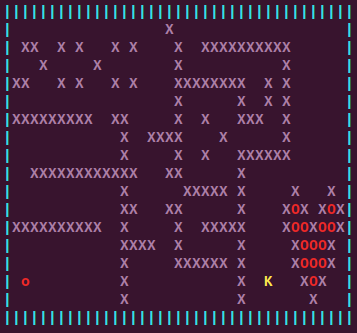
\includegraphics[scale=0.6]{./images/stage1.png}
        \hspace*{1cm}  %% pour mettre un espace (horizontal) de 5cm entre les deux images
        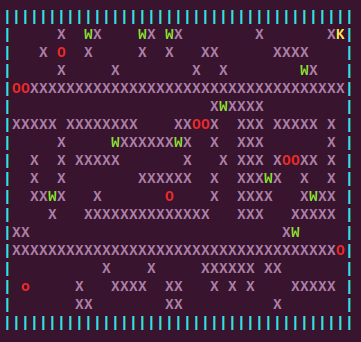
\includegraphics[scale=0.6]{./images/stageAlexD.png}
  }
        \end {figure}
        
         \begin {figure}[htbp]
        \hbox{ 
        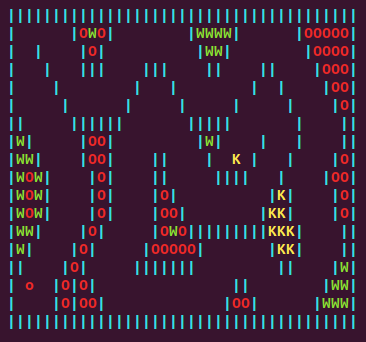
\includegraphics[scale=0.6]{./images/stageTitouan.png}
        \hspace*{1cm}  %% pour mettre un espace (horizontal) de 5cm entre les deux images
        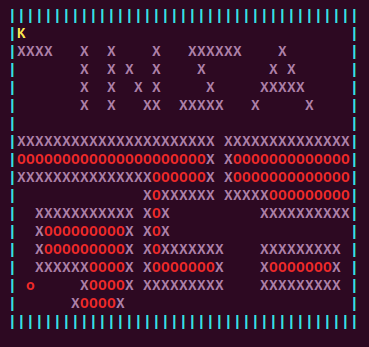
\includegraphics[scale=0.6]{./images/stageAlexO.png}
  }
  \end {figure}
  
  \begin {figure}[htbp]
        \hbox{ 
        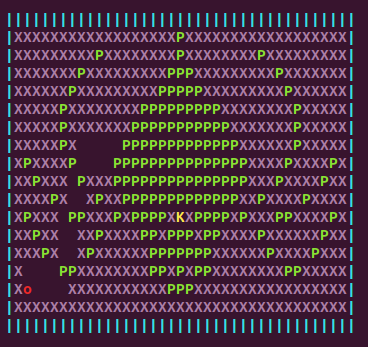
\includegraphics[scale=0.6]{./images/stageTim.png}
        \hspace*{1cm}  %% pour mettre un espace (horizontal) de 5cm entre les deux images
        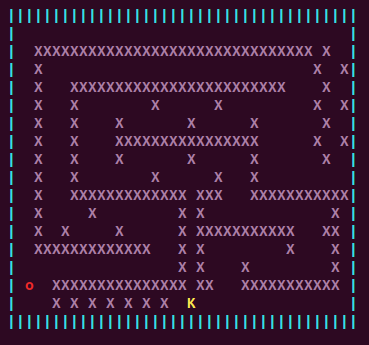
\includegraphics[scale=0.6]{./images/stageTom.png}
        
  }
  \end {figure}
  
  \centerline{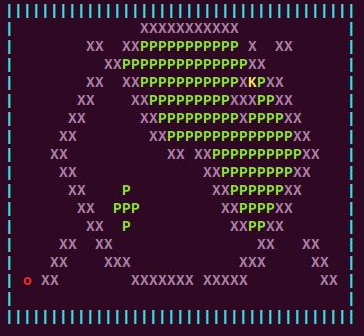
\includegraphics[width=0.5\textwidth]{./images/stageYassine.png}
        }
        
        \begin{algorithm}
        \Proc{RemplirPlateauSTAGE(E/S: plateauJeuStage: Plateau; fichierStage : fichier Texte; E : nomfichier: Chaîne de caractères)}{}
        \Proc{initStage(E/S xtaille,ytaille : Entier; vitesse : Entier; clignotement,findepartieStage : Booléen; serpNiveauParallèle : Serpent)}{}
        \Proc{estMortStage(E : objet : Contenus; E/S finpartieStage : Booléen)}{}
        \Proc{jouerPartieStage(E: clignotement : Booléen ; plateauJeuStage : Plateau; findepartieStage : Booléen; vitesse : Eniter; serpNiveauParallele : Serpent; xtaille,ytaille : Entier; E/S : scoore : Score; objetFinal : Contenus)}{}
        \Proc{traitementObjetFinal(E/S: objetFinal: Contenus; scoore: Score)}{}
        \Fun{choixFichierStage() : Chaîne de caractères}{}
        \Proc{jouerStage(E : xtaille,ytaille : Entier; vitesse : Entier; clignotement,findepartieStage : Booléen; serpNiveauParallele : Serpent; E/S : scoore : Score)}{}
        \end{algorithm}
        
       
    \newpage
    
    \subsection{Conception détaillée}
       Dans cette partie, nous allons revenir sur quelques détails techniques qu'il a codé et qu'il souhaite élaircir. 

        \subsubsection{Explications concernant les initialisations et le menu principal}

        \textit{\textbf{Les Initialisations }}\\
       Tout d’abord, nous allons expliquer comment les initialisations sont gérées, en effet une unité initialisation.pas qui est composée principalement de plusieurs procédures qu’on a rassemblées ensuite dans la procédure principale InitPartie: 

 - initSerpent qui initialise la taille et la position initiale du serpent qui correspond au centre du plateau.
 - initScore qui initialise le score de la partie à zéro et donne un nom au joueur en vérifiant que la chaîne de caractère n'est pas vide.
 - initiTaille de Plateau  qui permet d'initialiser la taille du plateau du jeu, en demandant à l'utilisateur de choisir entre trois niveaux, qui correspondent aux 3 choix de tailles prédéfinis par nous-mêmes après plusieurs tests sur le terminal pour éviter des problèmes de décalage de caractère  etc...
 - initDifficulteVitesse qui initialise  la vitesse de déplacement de serpent et qui s’agit du nombre des millisecondes.  L’ utilisateur doit choisir entre 3 vitesses prédéfinies.
  - la procédure initPlateau où on remplit un tableau de deux dimensions par des 'cases vides' et sans oublier le contour du plateau qui sont des 'cases murs' 


Ensuite pour le menu, on a choisi un type objet utilisé pour construire des types données complexes qui contiennent à la fois les fonctions et des procédures.
   
   \small
         \begin{lstlisting}[language=Pascal,frame=single,caption=Code source de l'unité les menus]
Type TMainMenu = object	
        Selectionner : integer;				
        MenuItems : array[0..3] of string; 
        {Tableau contenant les differents Propositions de Menu}	
        procedure AfficherMenu();
						
        procedure CurHaut(); {Curseur Haut} 
        procedure CurBas();  {Curseur Bas}
				
        function GetSelectionner(): integer; 
            end;
         \end{lstlisting}
  
Avec la fonction Read Key () de l'unité Crt on a pu lire le contenu de la touche entrée sur le clavier. A l'aide d'une boucle ‘case of’  on exécute, en fonction de ce que l'utilisateur a sélectionné, les différentes procédures proposées (soit les items de notre menu). Cela avec des conditions sur le curseur et quelques tests pour ne pas et dépasser la taille de ce menu.\\

  \small
         \begin{lstlisting}[language=Pascal,frame=single,caption=Code source de la procédure CurHaut() et CurBas()]
procedure TMainMenu.CurHaut();
	begin
		if Selectionner > 0 then Dec(Selectionner);
	end;
	
procedure TMainMenu.CurBas();
	begin
		if Selectionner < 3 then Inc(Selectionner);
	end;
         \end{lstlisting}

        \normalsize
       


        \subsubsection{Explications concernant la génération}
        
         \textit{\textbf{Processus général}}\\
        Dans un premier temps, nous tirons aléatoirement des coordonnées dans le plateau avec les fonctions : randomcoorX(xtaille) et randomcoorY(ytaille). Pour les rendre fonctionnelles pour tout type de plateau, celles-ci prennent en entrée la taille en x ou en y du plateau. 
        Nous ne pouvons générer un objet sur le plateau au hasard. Nous devons vérifier que la case n’est pas déjà occupée. Pour cela nous générons des coordonnées jusqu’à temps qu'elles respectent les conditions (quelObjet(xr,yr,tab)=vide) et (NoSerpent(xr,yr,serp)=Vrai).\\- quelObjet ressort la nature du Contenus qui se trouve aux coordonnées fournies en      entrée.\\
        - NoSerpent vérifie que le corps du serpent ne se trouve pas aux coordonnées fournies en entrée.\\Ains, nous sommes sûr de générer un objet sur une case libre.\\


        \textit{\textbf{Génération de fruits }}\\
        Afin de varier l’apparition des fruit, chaque aliment à une probabilité propre d’apparaître.
        Pour cela, nous utilisons la fonction randomFruit().
        Celle-ci tire aléatoirement un naturel entre 1 et 105. Un case of  déterminera ensuite le fruit à générer. 
        Voici un exemple pour illustrer notre méthode. 
       \small
         \begin{lstlisting}[language=Pascal,frame=single,caption=Code source la procédure randomFruit]
        randomint:=1+random(105); //prend une valeur entre 1 et 105 inclus
            case randomint of            
                1..21 :randomFruit:=pomme;   	//proba= 22%
                22..33:randomFruit:=orange; 	//proba= 11%
                34..47:randomFruit:=citron;	//proba= 13%
                ...
                ...
     
         \end{lstlisting}

        \normalsize
        Ici si le naturel tiré au hasard est 18 alors le fruit sera « pomme ».\\

        \newpage
         \textit{\textbf{Génération d'obstacles }}\\
        Cette génération fonctionne globalement comme la génération de fruits. Seulement, elle possède deux particularités supplémentaires.\\ 
        Dans un premier temps, rappelons par exemple que l’orange est un fruit très avantageux car il rapporte 200 points. Pour qu’il soit plus difficile de l’attrape, nous générons un obstacle proche de sa position.
        Nous utilisons alors la procédure RechercherObjet(). Celle ci recherche un objet (ici une orange, et s’il est sur le plateau, retourne sa position et le booléen FruitPresent=Vrai. \\
        Dans ce cas, nous générons un obstacle proche de cette position grâce à la fonction randomDistance(). 
        randomDistance() ressort un entier variant de -2 à +2. Ainsi la position de l’obstacle sera dans un cercle de rayon 2 centré sur l’objet .  \\
        Si l’objet n’est pas présent on génère aléatoirement l’obstacle.
        Dans un deuxième temps, nous effectuons une vérification supplémentaire. Nous vérifions que l’obstacle généré ne se situe pas proche de la tête du serpent afin d’éviter une mort immédiate. La fonction NoTeteSerpent() le permet.  
        
        \small
  \begin{lstlisting}[language=Pascal,frame=single,caption=Code source de la procédure générationObstacle]
RechercherObjet(tab,xtaille, ytaille, orange, xfruit, yfruit, fruitPresent); 
repeat 
begin
    if fruitPresent then
    begin
        xo:=xfruit+randomDistance();
        yo:=yfruit+randomDistance();
    end
    else
    begin			
        xo:=randomcoorX(xtaille);
        yo:=randomcoorY(ytaille);
    end;
end;
until ((quelObjet(xo,yo,tab)=vide) and DansPlateau(xo,yo,xtaille,ytaille)
and (NoSerpent(xo,yo,serp))) and (NoTeteSerpent(xo,yo,serp));
tab[yo,xo]:=obstacle;

\end{lstlisting}
\normalsize
        
        
         \textit{\textbf{Génération de tunnels }}\\
        Rappel :  le tunnel possède deux portes. En passant sur une porte le serpent se téléporte au niveau de l’autre porte. 
        Nous aurions pu générer simplement les portes en les plaçant aléatoirement sur le plateau. Seulement le principe du tunnel perd tout son intérêt si deux portes se situent à côté.  C’est pourquoi nous avons fait autrement.
        Nous avons coupé le plateau en 4 parties. D’abord on tire aléatoirement un première partie du plateau dans le laquelle nous générons une première porte.  Puis on génère l’autre porte en piochant à nouveau une partie du plateau en excluant la précédente. Ainsi les portes seront toujours éloignées l’une de l’autre.
       
        \subsubsection{Explications concernant le grandissement du serpent}

Lorsque le serpent mange un fruit, celui-ci voit sa taille augmenter d'une case. Pour cela il nous faut la procédure grandirSerpent ci-dessous. Comme elle contient beaucoup d'accès à des structures, nous allons l'expliquer en détail. Tout d'abord il faut connaître la taille du serpent (grâce à obtenirTailleSerpent) et la stocker dans une variable appellée \textit{`` tailleserpent ''}. Ensuite il nous faut aussi stocker la postition de la tête du serpent dans \textit{`` positionajout ''} car c'est à partir de celle-ci que nous allons pouvoir ajouter des cases à notre serpent. 

        \small
  \begin{lstlisting}[language=Pascal,frame=single,caption=Première partie du code source de la procédure grandirSerpent]
procedure grandirSerpent(dir : Direction; objet : Contenus; var serp : Serpent);

var positionajout : Position;
var tailleserp : Integer;

begin 

tailleserp:=obtenirTailleSerpent(serp);
positionajout:= obtenirCoordonneesCorpsSerpent(serp,1);

  \end{lstlisting}
  
  
  \normalsize
  Après cela, la procédure verifie si l'objet rencontré fait bien partie de la liste des fruits. Si c'est le cas, le sous programme fixe la nouvelle taille du serpent en rajoutant une case à la taille initiale. En fonction de la direction d'où vient le serpent lorsque qu'il rencontre le fruit, la case ajoutée aura des coordonnées différentes:

\begin{itemize}
 \item Haut : on ne change pas la coordonnée en X, on ajoute 1 à la coordonnées en Y
 \item Bas : on ne change pas la coordonnée en X,on enlève 1 à la coordonnées en Y
 \item Droite : on enlève 1 à la coordonnée en X, on ne change pas la coordonnées en Y
 \item Gauche : on ajoute 1 à la coordonnée en X, on ne change pas la coordonnée en Y
\end{itemize}
Pour finir, on attribue ces nouvelles coordonnées à la dernière et nouvelle case de notre serpent d'indice égal à la nouvelle taille du serpent (\textit{obtenirTailleSerpent(serp) = tailleserp+1}).
\small
  \begin{lstlisting}[language=Pascal,frame=single,caption=Deuxième partie du code source de la procédure grandirSerpent]
if objet in [pomme,orange,citron,coco,piment,weed] then
begin
	fixerTailleSerpent(tailleserp +1,serp);
	
	case dir of
	
	up : fixerCoordonneesCorpsSerpent(obtenirCoordonneeX(positionajout),
	obtenirCoordonneeY(positionajout)+1,obtenirTailleSerpent(serp),serp);
	
	down : fixerCoordonneesCorpsSerpent(obtenirCoordonneeX(positionajout),
	obtenirCoordonneeY(positionajout)-1,obtenirTailleSerpent(serp),serp);
	
	right : fixerCoordonneesCorpsSerpent(obtenirCoordonneeX(positionajout)-1,
	obtenirCoordonneeY(positionajout),obtenirTailleSerpent(serp),serp);
	
	left : fixerCoordonneesCorpsSerpent(obtenirCoordonneeX(positionajout)+1,
	obtenirCoordonneeY(positionajout),obtenirTailleSerpent(serp),serp);
	end;
end;
end;
\end{lstlisting}
\normalsize
        
        
        \subsubsection{Explications concernant les déplacements du serpent}
        
         \textit{\textbf{Lecture du clavier}}\\
        
        Dans le Snake, on déplace le serpent à l’aide des touches du clavier z,q,s,d. Il fallait donc que notre programme puisse lire ces touches entrées par l’utilisateur au cours du jeu. La procédure principale rendant ce processus possible est selectionTouche, et nous allons expliquer comment elle fonctionne.
        \scriptsize
                 \begin{lstlisting}[language=Pascal,frame=single,caption=Code source de la procédure selectionTouche]
                 
procedure selectionTouche(var toucheDirection : char; var dir : Direction; objet : Contenus);

var x:char;
var directionInterdite : Direction;
var dirtemp : Direction;
var derniereTouche : Char ;

begin
	directionInterdite := sensInterdit(dir); 
	derniereTouche := toucheDirection;
	toucheDirection := SelectionChar(derniereTouche);

	directionOpposee(objet,toucheDirection);							  
	dir := transformerToucheEnDirection(toucheDirection); 
	if dir = directionInterdite then 
		dir := sensInterdit(dir);	
		
	while keypressed() do 
		x:=readkey();	  
end;
                 
                \end{lstlisting}
         \normalsize

(Description des paramètres :         
toucheDirection est la touche du clavier saisie par l'utilisateur.
dir permet d'avoir la précédente direction du serpent et de sortir la direction traitée.
objet correspond à l'objet rencontré par la tête du serpent pour savoir si c'est une coco et ainsi inverser les touches directionnelles.)


selectionTouche commence par calculer la ``direction interdite'' : le serpent ne peut pas se retourner sur lui-même, il faut donc prévoir ce cas avant, car on la calcule à partir de la précédente direction du serpent et non pas à partir de celle que l'on s'apprête à entrer. Cela se fait grâce à la fonction sensInterdit qui à partir de la direction entrée en paramètre retourne son opposée.

On va par la suite lire la touche entrée tout en s'assurant qu'elle soit comprise entre z,q,s et d grâce à selectionChar :
         \normalsize
                 \begin{lstlisting}[language=Pascal,frame=single,caption=Code source de la procédure selectionChar]                 
function SelectionChar(derniereTouche : char) : char;

Var
  Key : Char;
Begin
  Repeat
    Key := ReadKey;
    if not(Key in [UpKey,DownKey,LeftKey,RightKey]) then 
		Key := derniereTouche;
  Until Key in [UpKey,DownKey,LeftKey,RightKey];
  SelectionChar := Key;
End;
                 \end{lstlisting}
                 
            \normalsize
Remarque: la fonction readkey sort juste le caractère correspondant à la touche sur laquelle on vient d'appuyer (c'est un fonction de crt)

Si le serpent est sur une coco, directionOpposee va inverser les directions.
Ensuite, on attribue à dir la direction correspondant à la touche dernièrement entrée par l'utilisateur. Le passage du type char de la touche entrée au type direction se fait grâce à la fonction transformerToucheEnDirection.

Si jamais cette direction est la même que la direction interdite calculée auparavant, alors pour éviter que le serpent ne s'arrête mais continue d'avancer, on affecte à la direction en cours (qui est donc interdite), sa direction interdite (donc en fait sa direction opposée) pour obtenir la direction dans laquelle le serpent était entrain d'avancer.

Pour finir, selectionTouche est chargée de gérer le buffer, qui est la file d'attente des saisies.  Par exemple, si on appuie sur beaucoup de touches à la fois, elles "attendent leur tour" pour entrer dans la boucle dans ce buffer.Les 2 dernières lignes du code permettent de vider celui-ci. Pour éviter des problèmes de stockage, de touches appuyées simultanément et d'autres encore, on ne veut travailler que sur une touche saisie par l'utilisateur. Tant que l'utilisateur entre une touche après avoir saisie sa première touche, on lit celle ci avec readkey ce qui la fait sortir du buffer.

Voilà comment notre programme fait en sorte de lire les directions entrées tout en vérifiant qu'elles sont correctes.\\

         \textit{\textbf{Déplacement du serpent}}\\\\ 
Maintenant que le programme sait reconnaître quelle touche a été enfoncée, et quelle direction est attribuée à cette touche, il est alors nécessaire de bouger le serpent en fonction de celle-ci. Pour cela, l’idée que nous avons eu est de faire bouger dans un premier temps la tête du serpent, puis de faire suivre le reste du corps. On a pour cela besoin de la procédure avancerSerpent, qui appelle avancerCorps.
\scriptsize
        \begin{lstlisting}[language=Pascal,frame=single,caption=Code source de la procédure avancerSerpent]
procedure avancerSerpent(xtunnel1,ytunnel1,xtunnel2,ytunnel2 : Integer;objet : Contenus;
                        dir : Direction; var serp : Serpent;var coordtete : Position);
    
    var pas: integer;
                                                                                    
begin
pas:=1;
if (dir= up) then
begin
    coordtete:= obtenirCoordonneesCorpsSerpent(serp,1);
    if ((objet=tunnel1) or (objet = tunnel2)) then
    begin
    case objet of 
    tunnel1:fixerCoordonneesCorpsSerpent(xtunnel2,ytunnel2-1,1,serp);
    tunnel2:fixerCoordonneesCorpsSerpent(xtunnel1,ytunnel1-1,1,serp);
    end;
    end
    else
    fixerCoordonneesCorpsSerpent(obtenirCoordonneeX(coordtete),
    obtenirCoordonneeY(coordtete)-pas,1,serp);
    avancerCorps(coordtete,serp);
end;

if dir = down then
...
if dir = left then
...
if dir = right then 
...
end.
        
        \end{lstlisting}
        \normalsize
        (Note: l'utilisation des tunnels sera abordée plus tard dans la partie 1.4.6. On ne s'intéresse pour l'instant qu'aux déplacements basiques du serpent.)
        
Pour faire avancer la tête, on attribue à la variable coordtête de type Serpent les coordonnées de la tête à l’instant où la touche a été enfoncée. On utilise donc l’accesseur obtenirCoordonneesCorpsSerpent(), avec un indice de 1 pour la tête.
On peut ensuite modifier ses coordonnées grâce à l’accesseur fixerCoordonneesCorpsSerpent et faire en sorte que si la direction entrée est :
\begin{itemize}
 \item Haut : la coordonnée y de la tête diminue de 1;
 \item Bas : la coordonnée y de la tête augmente de 1;
 \item Droite : la coordonnée x de la tête augmente de 1;
 \item Gauche :  la coordonnée x de la tête diminue de 1.
\end{itemize}
Maintenant qu’une première partie du serpent s’est avancée, le reste du corps doit suivre.
 L’enjeu de cette opération est de réussir à faire en sorte que pour n'importe quelle direction et pour n’importe quel morceau du serpent (sauf la tête), celui-ci se déplace de telle manière que sa position devienne la position du morceau qui le précède (en terme d’indice dans le tableau de coordonnées représentant le serpent) avant que ce morceau ne soit lui-même déplacée . En effet, l’idée est de déplacer en premier la tête du serpent puis d’utiliser une boucle déterministe pour faire en sorte que chaque morceau prenne la position initiale du morceau qui le précède. En résumé, on déplace d’abord la tête puis le deuxième morceau prend l’ancienne place de la tête puis le troisième morceau prend l’ancienne place du deuxième et ainsi de suite. Voici ci-dessous un  schéma qui illustre ce mécanisme.\\\\
        
        \centerline{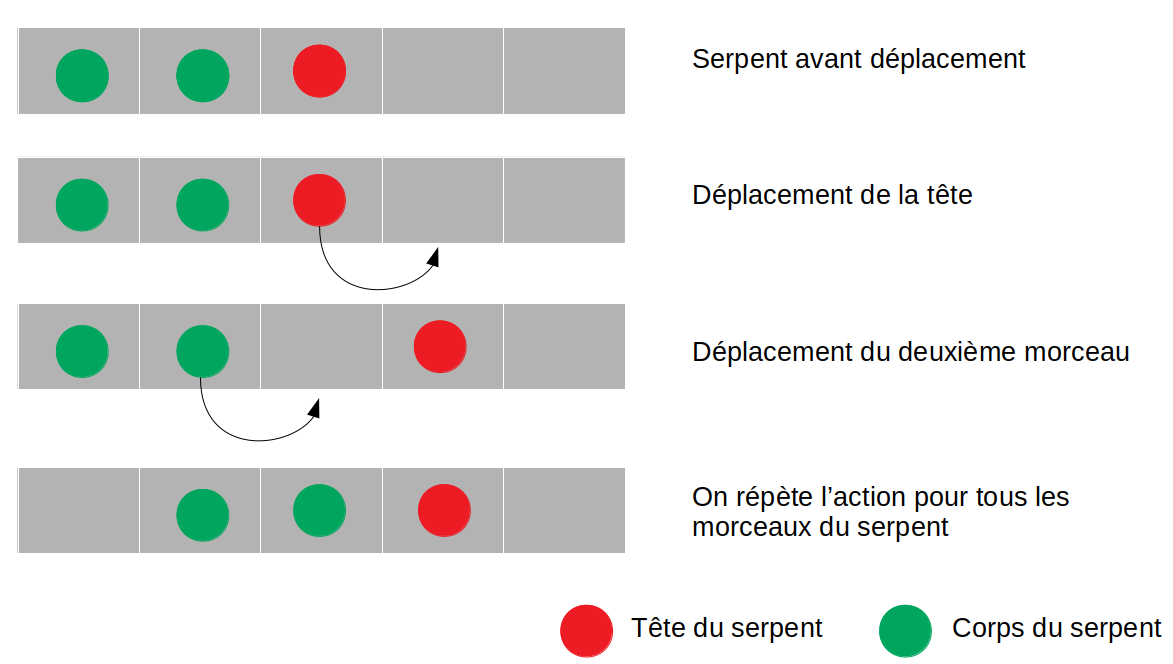
\includegraphics[width=0.6\textwidth]{./images/schemadeplacement.png}
        }
        \captionof{figure}{Schéma du mécanisme de déplacement du serpent}
        \vspace*{0.5cm}
        
        Au niveau de l’implémentation, il faut donc à chaque fois stocker dans une variable temporaire la position du morceau avant de la déplacer pour permettre le déplacement du morceau suivant. \\
        
        \begin{lstlisting}[language=Pascal,frame=single,caption=Code source de la procédure avancerCorps]
procedure avancerCorps(coordtete : Position; var serp:Serpent);

var i,tailleSerpent:Integer;
var coordtemp,coordtempcorps : Position;

begin
tailleSerpent:=obtenirTailleSerpent(serp);
coordtemp := coordtete;
    for i:=2 to tailleSerpent do 
        begin
            coordtempcorps := obtenirCoordonneesCorpsSerpent(serp,i);
            fixerCoordonneesCorpsSerpent(obtenirCoordonneeX(coordtemp),
            obtenirCoordonneeY(coordtemp),i,serp);
            coordtemp := coordtempcorps;
        end;
end;
        \end{lstlisting}
        
        \subsubsection{Explications concernant la gestion des scores}
        
        Nous allons expliquer comment les scores sont gérés lors de la réalisation d'une partie de snake.
        Tout d'abord, précisons que nous avons séparé les différents scores en fonction de la difficulté. 
        C'est pour celà que nous avons, dans notre dépot, 4 fichiers textes (\textit{ Score1, Score2, Score3, ScoreP}) contenant chacun les scores de la difficulté correpondante. Chaques fichier contient les 10 meilleurs scores ( Nom du joueur + nombre de points du joueur) jamais enregistrés.
        La gestion des scores se déroule en 2 étapes principales :
        
        \begin{enumerate}
         \item le chargement des scores dans un tableau à partir d'un des fichiers textes
         \item l'actualisation des scores (ajout ou non du scores enregistés lors de la partie)
         \item l'écriture des nouveaux scores dans le fichier
         
        \end{enumerate}
        
        Le chargement des scores se fait grâce à la procédure \textit{ChargerScore}. 
        \scriptsize
        \begin{lstlisting}[language=Pascal,frame=single,caption=Code source de la procédure ChargerScore]
procedure ChargerScores(vitesseEvo:Boolean; vitesse: Integer; var TabScore:TableauDeScore);
var 
	i, lueInt : Integer;
	lueStr : String;
	f : Text;
	
begin

if vitesseEvo then
begin
    Assign(f, 'ScoresP.txt')
end
else
begin
        Case vitesse of 
	300 : Assign(f, 'Scores1.txt');
	200 : Assign(f, 'Scores2.txt');
	100 : Assign(f, 'Scores3.txt');
	end;

end;

Reset(f);
for i := 1 to 20 do
	begin
	
	Readln(f, lueStr);
	FixerNomScore(lueStr,TabScore[i]);	
	Readln(f, lueStr);
	Val(lueStr, lueInt);
	FixerPointScore(lueInt,TabScore[i]);
	
	end;
	
Close(f);
end;
        \end{lstlisting} 

\normalsize
Tout d'abord, cette procédure assigne le bon fichier (en fonction de la vitesse) à la variable f. Si la variable booléen vitesseEvo est vraie, alors la vitesse choisit est celle progressive donc on asssigne à f le fichier correspondant à ce mode sinon on regarde les autres vitesses. Nous rentrons ensuite dans une boucle deterministe permettant de lire (en lecture avec "reset") le fichier. Ce dernier est conçu de façon à ce que la première chaine de caractère lue soit le nom du joueur, et la deuxième son nombre de points. Pour chaque joueur, les deux attributs de scores sont donc fixés dans le tableau de scores \textit{"TabScore"}.\\\\
Passons maintenant à l'actualisation des scores. Celle-ci se fait grâce à la procédure \textit{actualiserMeilleursScores}.
\scriptsize
\begin{lstlisting}[language=Pascal,frame=single,caption=Code source de la procédure acualiserMeilleursScores]
procedure actualiserMeilleursScores( vitesse : Integer; Nbpoint : Integer; nomJoueur : String;) 
var TabScore : TableauDeScore);
var 
i, j : integer;
Ajout : Score;
fichierMeilleursScores : Text;
actualise: boolean;

begin
i := 1;
fixerPointScore(Nbpoint, Ajout);
fixerNomScore(nomJoueur, Ajout);
actualise:= false;

while (i <= 10) and (actualise=false) do
begin
if (ObtenirPointScore(Ajout) >= ObtenirPointScore(TabScore[i])) then 
        begin
        
        If obtenirNomScore(TabScore[i]) = ObtenirNomScore(Ajout) then
        begin
        FixerPointScore(ObtenirPointScore(Ajout),TabScore[i]);
        actualise:= true;
        end
        
        else
        begin
        
        for j := 10 downto i do    
        
		begin
		fixerPointScore(obtenirPointScore(TabScore[j-1]),TabScore[j]); 
        fixerNomScore(obtenirNomScore(TabScore[j-1]),TabScore[j]); 
        end;
            
        FixerPointScore(ObtenirPointScore(Ajout),TabScore[i]);
        FixerNomScore(ObtenirNomScore(Ajout),TabScore[i]);
        actualise:= true;
        end
        end
        
	else i:=i+1;
end;

EcrireFichierTexte(vitesseEvo,vitesse,TabScore, fichierMeilleursScores);

end;
\end{lstlisting}
\normalsize

La procédure commence par fixer les deux attributs du score à ajouter (ou non ) dans le tableau de score \textit{TabScore}. Il est important de préciser que le tableau de score est trié dans l'ordre décroissant du nombre de points de chaque joueur. Commence ensuite une boucle indeterministe qui va permettre de modifier \textit{TabScore}. A chaque itération i , on regarde si le nombre de points du score à ajouter est supérieur à celui du score i du tableau. 

\begin{itemize}
 \item si le nombre de points du score à ajouter est inférieur à celui du score i, i devient i+1 et la boucle continue
 \item si le nombre de points du score à ajouter est supérieur, le tableau doit être modifié. Tout d'abord, si jamais le nom du score à ajouter est le même que celui du score i, seul le nombre de point sera modifié ( cela évite que quelqu'un totalement accro au snake monopolise tout le classement à lui tout seul :) ). Sinon, pour un rang j dans l'intervalle [i;10], on décale le score j. C 'est à dire que pour tout j, le score j se retrouve au rang j+1. Enfin on ajoute le score à ajouter au rang i.
\end{itemize}

Il ne reste plus qu'à écrire les scores du tableau dans le fichier texte correspondant. Prenant en entrée la vitesse, la procédure \textit{EcrireFichierTexte} nous permet de retranscrire les scores de TabScore dans le bon fichier texte. Elle est conçue de façon à écrire le nom et le nombre de points dans le bon ordre afin que les fichiers textes soient réutilisables par la suite.

        \subsubsection{Explications concernant les mécanisme de jeu d'une partie et d'un stage}
        
        \textit{\textbf{Mécanisme de jeu d'une partie}}\\
        
        Tout d’abord, il nous semble important de s’attarder sur la procédure jouerPartie de l’unité Jouer. C’est une procédure centrale de notre jeu. En effet, c’est à l’intérieur de cette procédure que se déroule le mécanisme de jeu. 
        
        \small
        \begin{lstlisting}[language=Pascal,frame=single,caption=Code source de la procédure jouerPartie]        
procedure jouerPartie(clingotement : Boolean; plateauJeu : Plateau;
findepartie : Boolean; vitesse : Integer; serp : Serpent;var xtaille,
ytaille : Integer; var scoore : Score);

var clignotement : Boolean;
var objet : Contenus;
var toucheDirection : Char;
var dir : Direction;
var fruit : Contenus;
var Xobjet,Yobjet,xtunnel1,ytunnel1,xtunnel2,ytunnel2 : Integer;
var ObjetPresent : Boolean; 
var mortSerp : Boolean;
var estVide : Boolean;
var xfruit,yfruit : Integer;
var detec : Contenus;
var vitesseInitiale : Integer;

begin 
    dir := right;
    objet := vide;
    detec := vide;
    vitesseInitiale :=vitesse; 
    affichaage(plateauJeu,scoore,serp,xtaille,ytaille,clignotement); 
    Repeat 
    begin
        selectionTouche(toucheDirection,dir,detec); 
        Repeat
        begin
            randomize(); 
            deplacementSerpent(xtunnel1,ytunnel1,xtunnel2,ytunnel2,dir,
            plateauJeu,serp,objet,mortSerp);
            clrscr();
            videPlateau(objet,xtaille,ytaille,plateauJeu,estVide); 
            affichaage(plateauJeu,scoore,serp,xtaille,ytaille,clignotement);
            jakadi(xtaille,ytaille,dir,collisionSerpent(serp),objet,serp,
            scoore,findepartie);
            detectionFruit(objet,detec);
            if estVide then 
                begin
                    vitesseWeedPiment(vitesseInitiale,objet,vitesse);
                    clignotement := doitClignoter(objet);
                    genererFruit(plateauJeu,xtaille,ytaille,serp);
                    genererObstacle(xtaille,ytaille,serp,plateauJeu);
                    genererTunnel(xtaille,ytaille,serp,plateauJeu, xtunnel1,
                    ytunnel1, xtunnel2, ytunnel2);
                    niveauStage(serp,plateauJeu,objet,scoore,xtaille,
                    ytaille,vitesse,clignotement);
                    affichaage(plateauJeu,scoore,serp,xtaille,ytaille,
                    clignotement);
                end;
                delay(vitesse);	
        end;
        until (keypressed() or (findepartie));
    end;
    until findepartie;
    vitesse := vitesseInitiale; 
end;
        \end{lstlisting}
        \normalsize
        On réalise premièrement quelques initialisations nécessaires au bon déroulement des appels présent dans cette procédure. On affiche ensuite un premier plateau de jeu avec les éléments initialisés lors de l’appel de la procédure d’initialisation de la partie effectué juste avant l’appel de la procédure jouerPartie. \\\\
        On rentre par la suite dans la boucle principale de cette procédure. C’est une boucle indéterministe qui a pour condition d’arrêt le booléen findepartie à Vrai. En effet, ce booléen est initialisé à Faux est pourra être modifiés lors de la partie. La première action que l’on effectue dans cette boucle est de récupéré la touche appuyé par l’utilisateur en s’assurant qu’elle soit valide à l’aide de plusieurs structures de contrôle au sein de la procédure selectionTouche. Une fois la touche entrée, on obtient donc une direction dans laquelle le serpent doit se déplacer continuellement jusqu’à ce que l’utilisateur n’appuie sur une nouvelle touche ou que la partie se termine.\\\\
        C’est donc pour cela que l’on entre dans une deuxième boucle indéterministe ayant comme condition d’arrêt « (keypressed() or (findepartie)) ». A l’intérieur de cette boucle, on utilise premièrement l’instruction « randomize() » et uniquement ici. Elle nous permet de pouvoir faire des générations aléatoires différentes à chaque fois que l’on utilisera l’instruction « random ». On réalise ensuite le déplacement du serpent en prenant en compte si le serpent traverse un tunnel ou s’il s’agit d’un déplacement classique. \\\\
        On appelle ensuite la procédure videPlateau qui permet de vider le plateau avant de procéder à de nouvelles générations et d’indiquer que si plateau a été vidé à l’aide d’un booléen. On appelle ensuite la procédure jakadi qui permet d’effectuer certaines actions en fonction de l’objet sur lequel le serpent vient de passer. En effet, Jakadi permet : de vérifier si le serpent est mort c’est-à-dire s'il rencontre un mur, un obstacle ou encore s’il rencontre sa queue ; d’augmenter le score si besoin ; de grandir le serpent si besoin ; d’appeler la procédure Renaissance qui va effectuer une action si l’objet sur lequel le serpent passe est une myrtille. On appelle ensuite une procédure detectionFruit qui permet de savoir si l’objet qui vient d’être rencontré par la tête du serpent est un fruit. Cette procédure procédure nous sert pour le mécanisme d’inversion des directions lorsque le serpent rencontre une noix de coco.\\\\
        On regarde ensuite si on vient de vider le plateau de jeu, dans ce cas cela veut dire que le serpent à rencontrer un fruit et on appelle donc les procédure qui gère les fruits weed, piment et citron. Par la suite, on génère donc un nouveau fruit, un nouvel obstacle et un nouveau tunnel. On appelle ensuite la procédure niveauParallèle qui permet de gérer le kiwi et donc l’entrée dans l’un des stages. On affiche ensuite le plateau après ces nouvelles générations. \\\\
        On stoppe ensuite le programme un certain temps correspondant à la vitesse. Ce mécanisme est décrit plus précisément dans les difficultés rencontrées.\\\\
        Enfin une fois la partie terminée, on prend soin de réaffecter à la variable vitesse la valeur de la vitesse initiale que l’on a stocké au début de cette procédure puisque l’on va avoir besoin de la valeur initiale de la vitesse pour stocker le score final dans l’un des différents fichiers selon cette vitesse.\\\\

        
        Concernant les déplacements, on peut rapidement s’intéresser au fonctionnement des tunnels. Grâce au mécanisme de déplacement que nous avons réalisé, l’utilisation des tunnels est relativement simple. En effet, il suffit de connaître les coordonnées des deux morceaux du tunnel pour pouvoir déplacer la tête du serpent au bon endroit lorsqu’elle arrive sur un morceau du tunnel.\\\\
        Pour nous faciliter la tâche, nous avons choisi de faire deux éléments distincts tunnel1 et tunnel2 dans le type contenus pour désigner les deux morceaux du tunnel. Dès lors, une fois que le serpent arrive sur un morceau du tunnel on sait grâce aux coordonnées du serpent de quel morceau il s’agit. On peut donc envoyer la tête du serpent vers l’autre morceau de tunnel en assignant aux coordonnées de la tête les coordonnées du deuxième morceau de tunnel. Une fois cela fait, le mécanisme est terminé puisque, comme décrit juste avant dans le mécanisme de déplacement du corps du serpent, le corps va suivra la tête est donc passer dans le tunnel morceau par morceau. \\\\
        
        \textit{\textbf{Mécanisme de jeu d'un stage}}\\
        
        Enfin, on peut d’intéresser de plus près au mécanisme des stages. Le pont entre la partie en elle-même et l’entrée dans le mécanisme de stage se fait grâce à la procédure niveauStage de l’unité Jouer.\\\\
        Pour le jouer le stage, on décide de garder certaines variables de la partie en les modifiant temporairement pour jouer le stage. En effet, comme énoncé dans la description du stage, les paramètres du stage sont toujours les mêmes quelque soient les initialisations de la partie. On a donc juste à affecter temporairement ses valeurs aux variables de la partie pour pouvoir ensuite réutiliser des procédures de l’unité Jouer utilisées dans la procédure JouerPartie. \\\\
        Voici comment se déroule le mécanisme de stage dans les grandes lignes. On commence à faire les initialisations nécessaires au stage. Ensuite, on rentre dans la procédure jouerStage et on  commence par charger l’un des plateaux de stage conçu par les membres du groupe (celui ci-étant stocké dans un fichier). On affiche alors un premier plateau avec le niveau à jouer. Puis on lance une procédure de jeu conçue de la même manière que la procédure jouerPartie en gardant seulement  les éléments qui nous intéresse pour jouer le stage. \\\\
        En effet, il faut préciser que le stage est un niveau de difficulté et donc nous avons décidé que les fruits ne servent que de décorations et ne peuvent donc pas être mangé par le serpent (cela signifie que le serpent passe dessus comme si la case ne contenait rien). Par la suite, si jamais le joueur est parvenu à atteindre le kiwi en or, on augmente son score directement dans le mécanisme de stage et non pas dans la procédure d’augmentation du score appelé dans jouerPartie.\\\\
        Enfin, on sort alors de la procédure jouerStage puis on prépare le retour à la partie dans la fin de la procédure niveauStage avec un décompte et un affichage du plateau tel qu’il va être quand le jeu va reprendre. \\\\
        
        \newpage
        \section{Difficultés rencontrées}
        
        Lors de ce projet nous avons dû faire face à plusieurs difficultés techniques, c’est-à-dire des difficultés liées à l’implémentation du code.
        
        \subsection{Gestion des générations aléatoires}
        \setlength{\parindent}{1cm}
        Premièrement, l’un des problèmes que nous avons rencontré résidait dans la gestion des générations aléatoires. En effet, pour pouvoir jouer une partie correctement, nous avons besoin de générer plusieurs éléments comme les fruits, les obstacles ou encore les tunnels tout en vérifiant certaines conditions comme par exemple le fait qu’il n’y ait pas de morceau du serpent à l’endroit où l’on souhaite générer. Cela implique donc l’utilisation de boucles indéterministes pour générer des coordonnées jusqu’à ce que toutes les conditions soient vérifier.\\\\
        Dans toutes les fonctions et procédures de générations nous avions donc placé l’instruction « randomize() » permettant les générations aléatoires à l’aide de l’instruction « random ». Cependant, le fait de mettre la commande « randomize() » à plusieurs endroits différents dans le code a provoqué un blocage dans  la génération aléatoire. Les éléments générés aléatoirement étaient toujours les mêmes pendant un grand nombre de tirages ce qui entraînait donc des boucles indéterministes très lentes. Par conséquent, le jeu subissait de gros ralentissements à chaque fois que nous devions générer un nouvel élément. Pour solutionner ce problème, nous n’avons donc mis l’instruction qu’une seule fois dans la procédure jouerPartie.
        
        \subsection{Gestion des saisies au clavier}
        \setlength{\parindent}{1cm}
        De plus, un autre problème que nous avons rencontré était de faire en sorte que la partie ne soit pas perturbée par un appui sur une mauvaise touche du clavier. Nous avons dû faire face à deux soucis dans le cadre de ce problème : le premier était de faire en sorte que le serpent continue d’avancer dans la dernière direction qui lui a été donné lorsque le joueur appuie sur la touche opposée à cette direction (c’est-à-dire que le joueur tente d’aller dans ce que nous avons appelé la direction interdite) ; le deuxième était de faire en sorte que le serpent continue dans la dernière direction qui lui a été donné lorsque le joueur appuie sur une touche qui ne fait pas partie des touches directionnelles (pour nous ZQSD). \\\\Pour résoudre le premier sous-problème, lorsque nous détectons que le joueur tente d’aller dans la direction interdite (qui est calculée à partir de la direction précédente) alors nous affectons la direction précédente que nous avons gardé en mémoire (et qui est donc valide) à la place de la direction interdite. De la même manière, pour résoudre le deuxième sous-problème, lorsque nous détectons que la touche sur laquelle le joueur appuie n’est pas une des touches directionnelles prévues, alors nous affectons à la touche lue la valeur de la dernière touche valide à la place de la touche incorrecte. En effet, si nous n’effectuons pas ces deux manipulations le serpent se stoppe puisque la sélection d’une touche valide (et donc d’une direction valide) se fait à l’aide d’une boucle indéterministe ayant pour condition d’arrêt le fait que la touche entrée soit valide. La condition de sortie de cette boucle n’était donc pas remplie et la boucle était donc en attente d’une nouvelle saisie ce qui stoppait le serpent dans son déplacement.
        
        \subsection{Gestion de la continuité du déplacement du serpent}

        Par ailleurs, nous avons aussi rencontré des difficultés pour faire en sorte que le serpent continue de se déplacer dans la direction qui lui est donnée sans que le joueur n’est à appuyer à chaque fois sur la touche. En plus de cela, nous devions aussi prendre en compte la fonctionnalité de vitesse que nous avons décidé de réaliser. L’astuce réside alors dans le fait que nous utilisons la fréquence d’affichage pour faire avancer le serpent tout seul dans la direction demandée mais aussi pour le faire avancer plus ou moins vite. \\\\ En effet, le programme enchaîne très rapidement les avancées du serpent en terme de coordonnées, il suffit donc de jouer avec des affichages placés au bon endroit pour donner un aspect fluide au jeu mais aussi avec les délais entre les affichages qui permettent donc de faire avancer le serpent pus vite si le délai est plus court ou plus lentement si le délai est plus long. Tout ce mécanisme se déroule dans la boucle principale de la procédure jouerPartie. Pour stopper le programme juste après l’affichage (c’est-à-dire pour réaliser le délai entre les affichages successifs puisque le reste des instructions est exécuté bien trop rapidement), on utilise la procédure « delay » de l’unité Crt. On lui passe alors en entrée notre variable vitesse correspondant au temps d’attente en millisecondes. En faisant varier la variable vitesse, on fait alors varier la le temps d’attente entre les affichages et donc la vitesse de déplacement du serpent à l’écran. \\\\
        
        \newpage
        \hfill
        \section{L'impact de l'utilisation des outils de gestion de projet informatique}
       
        \subsection{Git}
       
        \setlength{\parindent}{1cm} % Définit la largeur de l'alinéa à 1 cm.
        
        Contrairement au précèdent projet informatique réalisé dans le cadre du cours de I2, nous avons eu en notre possession des outils qui nous étaient inconnus mais qui ont énormément facilité la tâche pour mener à bien ce projet. L'outil de gestion qui nous a été le plus utile, et même essentiel, est \textit{\textbf{Git}} qui est un logiciel de gestion de versions décentralisés. Il permet de faire du partage de fichiers en ligne, c'est-à-dire que chaque personne du projet peut modifier les fichiers qui sont sur le dépôt et chacun peut ensuite, après une simple commande, avoir la mise à jour automatique sur sa machine des fichiers modifiés par un autre utilisateur. Alors que dans nos projets précèdents il était difficile et long de s'envoyer du code (mail, filezilla ..) et de mettre à jour nos fichiers correctement, \textit{\textbf{Git}} nous a rendu très facile le partage de code (surtout durant la période de confinement) et la vitesse de réalisation du projet a décuplé grâce à cela. 
        
        \subsection{Dia}
        
        \setlength{\parindent}{0cm}
        Le second outil qui nous a grandement aidé est un logiciel libre de création de diagramme : \textit{\textbf{Dia}}. Celui-ci nous a permis de créer notre analyse descendante beaucoup plus facilement qu'avec d'autres logiciels comme LibreOffice Draw par exemple. En effet, l'environnement de \textit{\textbf{Dia}} ainsi que ses fonctionnalités sont vraiment adaptées pour réaliser des analyses descendantes de taille importante comme c'est le cas dans ce projet.

        \subsection{Kile}
        
        Enfin pour réaliser notre rapport, nous avons utilisé le logiciel \textit{\textbf{Kile}} qui est un éditeur de texte pour les documents écrits en LaTeX. L'intérêt de \textit{\textbf{Kile}} dans la rédaction est que ce logiciel permet de voir à chaque compilation du code ce que celui-ci donne en format pdf. En effet, la partie gauche du logiciel est le code et la partie droite la version compilée. On a donc un suivi en temps réel des modifications du texte directement sur la partie droite ce qui est un gain de temps significatif. De plus, grâce au template de rapport fournit par nos enseignants, nous avons pu nous familiariser avec le langage LaTeX et apprendre les commandes de base pour réaliser un rapport.\\\\
         Pour communiquer textuellement et vocalement entre nous à distance (merci covid) nous avons utilisé \textit{\textbf{Discord}}. 
        
        \subsection{Avantages}
        
        Pour conclure, tous ces outils nous ont permis:
        
        \begin{itemize}
        \item d'avoir une meilleure organisation 
        \item de faciliter nos échanges 
        \item d'accroître notre vitesse de réalisation
        \item d'obtenir des bases en \LaTeX{}
        \end{itemize}
        
        \section{Les impressions du groupe vis-à-vis du projet}
        
        \subsection{Conditions coronavirus}
        La situation sanitaire mondiale nous a obligée à travailler à distance et donc à utiliser les outils de gestion de projet dans un exercice plus vrai que nature. Malgré le fait que nous ne pouvions pas se voir à l'INSA, nous avons su tenir notre planning de travail dans ce contexte inédit.
        
        \subsection{Dynamique de groupe}
        Il y a une bonne entente au sein du groupe, c'est un groupe dynamique et réactif dans les tâches à réaliser. La customisation ``à la carte'' de la version originale du snake a permis aux plus créatifs d'entre nous de trouver de belles idées que nous avons réussi à mettre en oeuvre tous ensemble. \\ 
        En règle général, il était très agréable de travailler sur ce projet. Chacun était libre de choisir sa partie, sa gestion du travail et de créer librement.  
        
        \subsection{Points positifs}
        La prise en main de ces nouveaux outils à travers ce projet informatique est un véritable avantage dans une formation d'ingénieur. Certes, nous avons découvert ces outils sous un angle informatique néanmoins il est évident qu'ils nous seront très utiles quelque soit le domaine d'ingénieurie suivi. \\
        Dans un second temps, nous ressentons une réelle progression au niveau de la gestion d'un projet de genre.
        Nous avons reussi à fournir un travail continue. Nos réunions quasi-hebdomadaires sur discord nous ont permis d'échanger un maximum et donc de gagner un temps précieux: certains problèmes ont pu être résolus rapidement et nous avons pu nous entraider efficacement via des partages d'écran.
        
        \subsection{Points négatifs}
        Les outils abordés sont relativement complexes à prendre en main mais nous nous sommes tous habitués à les utiliser tout au long de ce projet. De plus, nous avons su nous entraider afin d'améliorer notre maîtrise sur les différents logiciels. 
        
        \newpage

\section{Conclusion}

En conclusion, ce projet fut l‘occasion d'exploiter nos compétences acquises lors de nos enseignements à l’INSA.\\

	A travers la réalisation d’un jeu relativement simple, nous avons appris à maîtriser de nouveaux outils tout en professionnalisant nos méthodes de travail. L’utilisation du Latex pour une rédaction propre et efficace, de Git pour une bonne gestion de nos fichiers et le respect d’une méthodologie propre à la création d’un programme informatique furent ainsi les clés de la réussite de ce projet. Il est clair que ces techniques de travail nous seront d’une grande utilité quelque soit la formation d’ingénieur envisagée.\\

	L’un des atouts de ce projet fut le travail d’équipe. En tant que futurs ingénieurs, il est important, si ce n’est nécessaire, d’être à l’écoute de ses coéquipiers et de savoir s’entraider pour surmonter les difficultés. Ainsi , travailler a plusieurs sur la réalisation du SNAKE nous a permis  d’acquérir des réflexes et des compétences, indispensables à notre formation. Ce projet nous a alors offert de solides bases  en terme de gestion de projet.\\

	Pour finir ce projet, nous voulions remercier notre mentor et mécène.  
	\begin{center}
	 
\includegraphics[scale= 0.25]{./images/DJSNAKE.jpg}  
	 \caption{DJ SNAKE notre sensei $\ddot\smile$}
    \end{center}


\section*{Sources} % L'astérisque est pour que la section ne soit pas numérotée
\addcontentsline{toc}{section}{Sources} % Cette commande ajoute la section à la table des matières malgré le fait qu'elle ne soit pas numérotée
    \begin{itemize}
        \item Photo de la page de garde: \url{https://res.cloudinary.com/jerrick/image/upload/c_crop,fl_progressive,h_630,q_auto,w_1200/o3lngeybtdpwnbgzlna2.jpg}
        \item Photo du DJ: \url{https://djsnake.com/wp-content/uploads/2019/10/image-url-6-1.jpg}
    \end{itemize}


\end{document}
